%===================================== CHAP 8 =================================

\chapter{Computational Study}


In this chapter, a computational study based on the solution approach outlined in Chapter 5 is presented. First, in Section \ref{sec:exact}, the optimal solution with perfect information is presented. Secondly, in Section \ref{sec:inexact}, the performance of each of different solution approaches are presented. 


The mathematical programming model is written in the algebraic modelling language Mosel and implemented in FICO\textsuperscript {\textregistered} Xpress Optimization Suite 8.3, using a HP EliteDesk 800 G3 DM 65W computer with Intel\textsuperscript{\textregistered} Core\textsuperscript{\texttrademark} i7-7700 3.6 GHz processor and 32 GB RAM. The operating system in use is Windows 10 Education 64-bit. The results obtained from Xpress are written to CSV files, which are exported to R to be further analyzed. 

\section{Solution with realized points}\label{sec:exact}
First, the initialization of sets and parameters are presented. Following is a presentation of the results from running the model with realized points. The last part of the section compares the results with top performing managers in FPL and analyzes their performance. 

\subsection{Initializations of parameters}    
%DEL1 
The sets and parameters described in Section \ref{def_sets_ind_par_var} are presented in table \ref{initialization_of_parameters}. 



\begin{table}[H] 
\tabcolsep=0.11cm
\label{initialization_of_parameters}
\centering
\caption{Initialization of parameters.}
\begin{tabular}{@{}lll@{}}
\toprule
Parameters                       &   &                                                                                                \\ \midrule
$\mathlarger{\rho_{pt}}$ & - & Realized points for a player $p$ in a gameweek $t$. \\
$\epsilon$                       & - & Set to 0.1.                                                                     \\
$\sigma_{1}, \sigma_{2}, \sigma_{3} $                     & - & Set to 0.01, 0.001 and 0.0001 respectively.                                               \\
$R$                              & - & 4 points deducted if number of free transfers is exceeded.       \\
$M^{K}$                          & - &  2 goalkeepers required in the selected squad.                                      \\
$M^{D}$                          & - &  5 defenders required in the selected squad.                         \\
$M^{M}$                          & - & 5 midfielders required in the selected squad.                                     \\
$M^{F}$                          & - & 3 forwards required in the selected squad.                                    \\
$M^{C}$                          & - & 3 players allowed to have from the same club.                                \\
$E$                              & - & 11 players required in the starting line-up.                              \\
$E^{K}$                          & - & 1 goalkeepers required in the starting line-up.                                       \\
$E^{D}$                          & - & 3 defenders required in the starting line-up.                  \\
$E^{M}$                          & - & 3 midfielders required in the starting line-up.                                 \\
$E^{F}$                          & - & 1 forward required in the starting line-up.                     \\
$B^{S}$                          & - & 100 million as starting budget.                                                                              \\
$\beta$                          & - & Set to 1.                                                                                  \\          
$\bar{\alpha}$                   & - & Set to 14.                                                                      \\

$\phi$                         & - & 3 players are substitutes.                                                         \\
$\phi^{K}$                   & - & 1 keeper among the substitutes.                                                          \\
$\overline{Q}$                   & - & 2 free transfers possible to accumulate over gameweeks.                                              \\
$\underline{Q}$                  & - & 1 free transfers given every gameweek.                                      \\ \bottomrule
\end{tabular}
\end{table}

The data on each player's sell price and buy price in a gameweek is collected from FPL's homepage \url{www.fantasy.premierleague.com}.
Nearly all the parameters are set according to the rules of FPL. 
\begin{table}[H]
\centering
\caption{Initialization of sets.}
\begin{tabular}{@{}lll@{}}
\toprule
Set           &   &                                                               \\ \midrule
$\mathcal{T}$ & - & 35 gameweeks,                                             \\
$\mathcal{P}$ & - & 625 players,                                               \\
$\mathcal{C}$ & - & 20 clubs,                                                 \\
$\mathcal{L}$ & - & \{1,2,3\}, where 1 is first priority, \\
$\mathcal{T}_{FH}$ & - & Gameweek 1 to 21 is in the first half of the season,\\
$\mathcal{T}_{SH}$ & - & Gameweek 22 to 35 is in the second half of the season.\\
\bottomrule
\end{tabular}
\end{table}


\begin{table}[H]
\centering
\caption{Computational statistics for the instance with realized points.}
\label{Computational statistics}
\begin{tabular}{@{}llll@{}}
\toprule
                            & Rows    & Columns & Elements \\ \midrule
Original Problem Statistics & 172 034 & 254 425  & 1 052 715  \\
Xpress Presolve Statistics  & 170 750 & 206 689  & 891 995   \\ \bottomrule
\end{tabular}
\end{table}



\begin{table}[H]
    \centering
    \caption{Problem size of exact solution method}
    \begin{tabular}{c|c}
        Total number of variables & Total number of constraints  \\
         & 
    \end{tabular}
\end{table}

\begin{figure}
    \centering
    \includegraphics{}
    \caption{figure of when the solutions are found after how long time.}
\end{figure}

\begin{table}[H]
    \centering
    \caption{Results of implementation of exact solution method.}
    \begin{tabular}{c|c}
        LP Bound & Best solution & Best bound & Gap  \\
         & &
    \end{tabular}
\end{table}


DEL 2: 
Figure \ref{Figure_Realized_points} gives an overview of how many points the model in chapter \ref{model_formulation} gets in every gameweek when solved with perfect information. The red dots represents gameweeks where the gamechips were used. The different gamechips were played in the following gameweeks: 

\begin{itemize}
    \item Wildcard no. 1 was used ahead of gameweek 11
    \item Wildcard no. 2 was used ahead of gameweek 26
    \item Bench Boost  was used in gameweek 12 
    \item Triple Captain was used in gameweek 31
    \item Free Hit was used in gameweek 21 
\end{itemize}

\begin{figure}[H]
\label{fig:Realized_points}
    \centering
    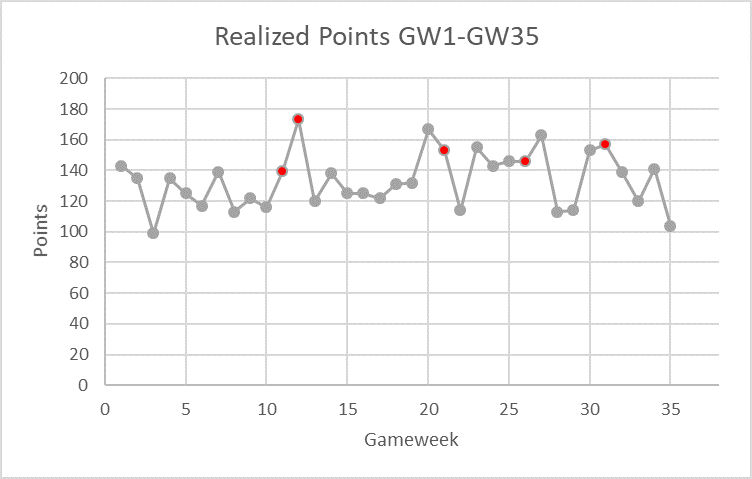
\includegraphics[scale=1.00]{fig/chapter_7/RealizedPoints.png}
    \caption{The graph shows the points per gameweek with perfect information}
\label{Figure_Realized_points}    
\end{figure}

We find it necessary to comment on the choices made for selecting when to play the gamechips. Firstly, the Wildcard no.1 was used one week ahead of the bench boost was played. This makes good sense at it is wisely to ensure that you have got 15 players that will earn lots of points when playing the Bench Boost. Further, the triple captain chip was used in gameweek 31 which is reasonable as Mohammed Salah scored 4 goals and had 1 assist in this particular gameweek, yielding a score of 29 points. This is was the highest score obtained in one gameweek by any Premier League players. Finally, the Free Hit chip was used in gameweek 21. This was a blank gameweek, containing only 9 fixtures as Tottenham and West Ham did not play. It is reasonable to assume that a free hit should be used either ahead of a blank or doble gameweek, to ensure that all your selected players are featured at least one match for that particular gameweek.
\newpar
Figure \ref{Figure_Transfers} shows how many transfers the model made in each gameweek. It is notable that the model performs most transfers when the Wildcards and the Free Hit are played. This makes sense as transfers are free when playing these gamechips. In general, one can say that the model makes many transfers compared to human managers. However, this is due to the fact that this is an optimal solution. Thus, it selects the players that over performed in a particular gameweek. Every gameweek there are some players that surprise the FPL managers. For instance, if a defender suddenly scores two goals in a match, the goals themselves represent 12 points. 

\begin{figure}[H]
\label{fig_Transfers}
    \centering
    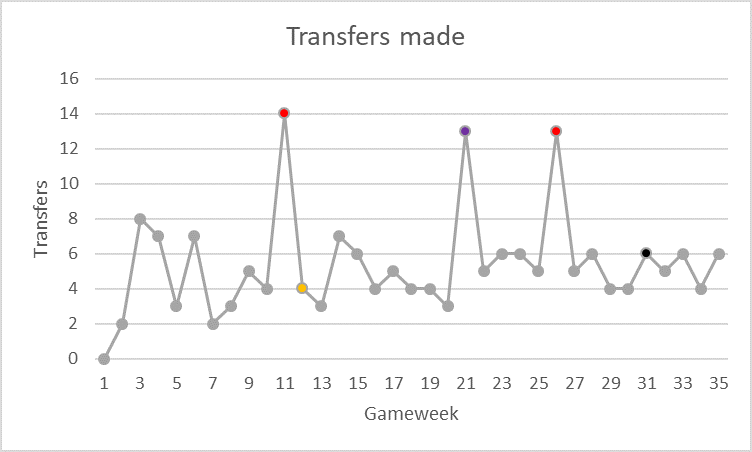
\includegraphics[scale=1.00]{fig/chapter_7/Transfers.png}
    \caption{The graph shows how many transfers the optimal solution makes in every gameweek}
\label{Figure_Transfers}    
\end{figure}


\begin{figure}[H]
\label{fig:Comparison}
    \centering
    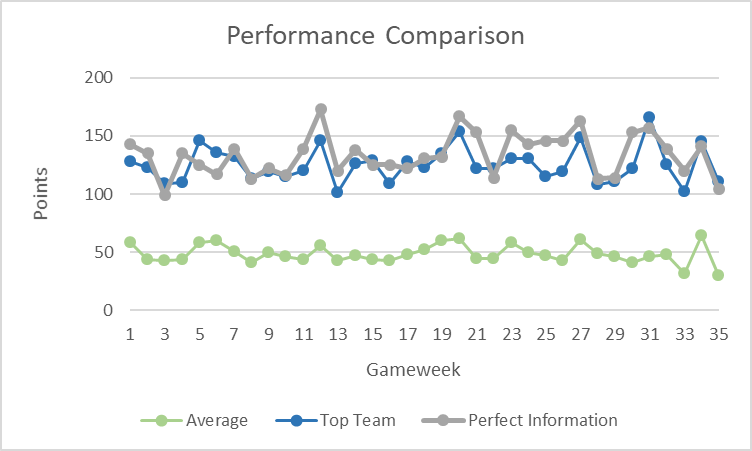
\includegraphics[scale=1.00]{fig/chapter_7/Comparison.png}
    \caption{The graph compares the average and top performer of each Gameweek to the optimal team with perfect information}
\label{Figure_Comparison}    
\end{figure}

Some readers may find value in comparing the optimal FPL solution to human managers. Figure \ref{Figure_Comparison} compares the optimal solution in every gameweek to the average performance of the human managers. In addition, it includes the maximum score obtained by a human in each gameweek. It is notable that the optimal solution performs well ahead of the average managers, scoring at least twice as many points in every gameweek. Further, it is worth noticing that the optimal overall solution may be beaten by the best manager in individual gameweeks. This is due to the fact that the optimal solution maximizes the points over the entire season, and not only over one particular gameweek. Further, managers that finish on top for a gameweek often use a gamechip in order to maximize their weekly score. 
\newpar
There seem to be some positive correlation between the optimal solution and both the weekly top performers as well as the average scores. From table \ref{Figure_Comparison} one can see that the average managers and the optimal solution have a tendency of moving in the same direction. Hence, when the optimal solution receive a high score, the average managers have a tendency of doing the same. This might be due to top rated players performing well in those particular gameweeks. For instance, if a player that has performed well over the entire season receives an abnormal high score, it is likely that the average will increase as most managers select this player. Consider Mohamed Salah, who has had an incredible season. At some point he was selected by more than 63\% of the human managers. Hence, if he had an outstanding gameweek, it is very likely that he's selected by both the optimal solution as well as by the average managers. Thus, when he performs well it is likely that both the average and the optimal solution earn numerous points. 
\newpar
As stated in chapter \ref{introduction} it is interesting to compare the optimal solution strategy to that of the manager of leads the overall ranking. Figure \ref{Top_Manager} provides a weekly overview of this comparison.

\begin{figure}[H]
\label{fig:Top_Manager}
    \centering
    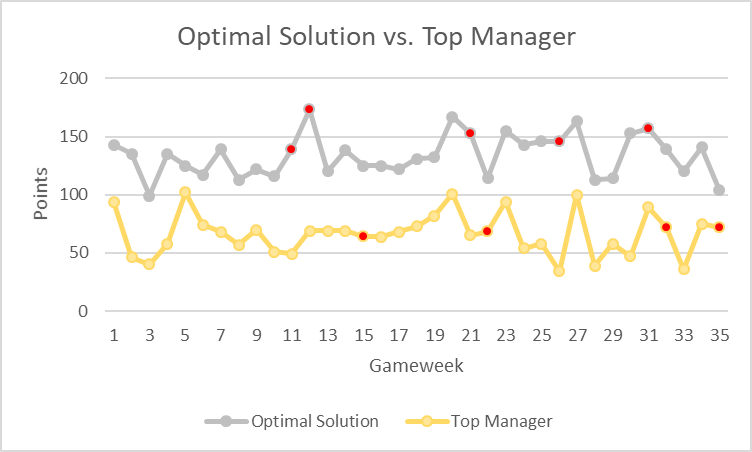
\includegraphics[scale=1.00]{fig/chapter_7/Top_manager.png}
    \caption{Comparing optimal solution strategy to top manger}
\label{Top_Manager}    
\end{figure}

As suggested in the introduction, the optimal solution strategy largely outperforms that of the top manager of Fantasy Premier League. In total it separates 2348 points between the two solutions, more than twice the amount of points gained by the top rated manager. It is notable that the two teams do not play their gamechips in any of the same gameweeks. The top manager played his triple captain in gameweek 22, where Tottenham and West Ham were featured twice. Selecting Harry Kane as his triple captain is an understandable choice, as Harry Kane was the top scorer of Premier League at that point of time. However, Kane under performed in both matches only receiving three points in total. In addition, one can see that the top manager played his second wildcard in gameweek 32, two weeks ahead of a double gameweek. Finally, he played his free hit in gameweek 35 which is reasonable as this was ahead of a blank gameweek. As expected, the two teams presented in figure \ref{Top_Manager} are positively correlated.   
 
Interesting points:
\begin{enumerate}
    \item picture of when the solutions are found after how long time. discuss 
    \item disc
    \item When are the chips used
    \item What is the difference between the best player and the optimal solution
    \item frequent formation
    \item How many substitutions
\end{enumerate}


\section{Solution with expected points}\label{sec:inexact}
\begin{enumerate}
    \item all the gamechips are explained before this chapter. the implementation of the gamechips do not change in each forecasting method. 
    \item a parameter study on the average method for horizon, penalty and obj.value on average forecasts on season 2016. This has been done before computational study. Suggestion figure: matrix for horizon and penalty, with green = good obj value, red = bad obj value
    \item  the decision on the threshold(risk) is explained in Experimental setup method. 
    \item INGENTING ENDRES I DETTE KAPITTELET. KUN DRØFTING AV RESULTATER. 
\end{enumerate}

\subsection{Preliminaries}
\subsubsection{Forecasting Error}
The forecasting error of the complete 2017/2018 season based on the two average-based models are summarized in Table \ref{tab:accuracy_average}. Note however, that it is not given that the method with lowest error will performed best. 

\begin{table}[H]
\centering
\caption{Summary of forecasting errors on the average methods}
\label{tab:accuracy_average}
\begin{tabular}{llll}
Method & ME & RMSE & MAE\\
Argentina & 0.00882 & 2.436 & 1.295 \\
Improved  & 0.0436  & 2.455 & 1.294 \\ 
Odds  & NA  & NA & NA   \\
Regression  & NA  & NA & NA \\
\end{tabular}
\end{table}


\subsection{Average}

tabell 1: total sum points etter uke 35, toal mean for hver runde, ranking. 

forklare minst og høyeste antall illegal transfers og referere til appendiks. 

graf 1: poeng hver runde, average for hver runde i selve spillet, når gamechippene brukes, 



Possible metrics: 

Results of total sum, average, predicted points pr round opp mot actual points pr round, computational time, st.dev highest round, lowest round, number of illegal transfers, when gamechips are used, "case-study"



\begin{table}[H]
    \centering
    \begin{tabular}{c|c|c|c|c}
        Round 10 - 20 & Points avg WITH NO variance & ill transfers WITH NO variance & Points avg WITH variance & ill transfers WITH variance\\
    \end{tabular}
    \caption{Results of avg no variance for round 10 -20.}
\end{table}

- Summarizing conclusion based on the variance/standard deviation of each method.
- Say something about the computational time for each method. 

\begin{table}[H]
\centering
\caption{Results of total sum, average, total sum best player. Model without variance.}
\begin{tabular}{llllll}
& Our Method & Our Method w/var  & Average Players & Best Player & Exact\\
Total sum  & NA  & NA & NA & NA & NA \\
\end{tabular}
\end{table}



\textit{Case-study of round w/chip to show that the model makes sense}

\subsubsection{Argentina}
 tabell 1: total sum points etter uke 35, total mean for hver runde, ranking. 

forklare minst og høyeste antall illegal transfers og referere til appendiks. 

graf 1: poeng hver runde, average for hver runde i selve spillet, når gamechippene brukes,


\subsubsection{Improved}


\subsection{Odds}
\subsection{Regression Model}
\subsection{Summary}

\section{Recommendations for human FPL managers}

- hvilke anbefalinger kan man gi til fpl managere? 
     * hvilke formasjon går igjen i løsningene. lønner det seg med forsvarsspillere eller angrepsspillere?  
    * er budsjettet alltid oppfylt? og hvordan utvikler verdien til laget seg over sesongen? 
    
    - Tabell over Formasjon i optimal solution. 

\begin{table}[H]
\centering
\caption{Results of total sum, average, total sum best player. Model without variance.}
\begin{tabular}{llllllll}
& Average Argentina & Average Improved & Odds & Regression  & Average Players & Best Player & Exact\\
Total sum  & NA  & NA & NA & NA & NA & NA & NA \\
\end{tabular}
\end{table}


\begin{comment}
Good discussion points: 
\begin{enumerate}
    \item hvis man legger restriksjon på formasjon. Hvilke formasjon gir mest poeng?
    \item når bruker man de forskjellige chippene, og hvor effektive er de?  
\end{enumerate}
\end{comment}

